% This file was created by tikzplotlib v0.8.5.
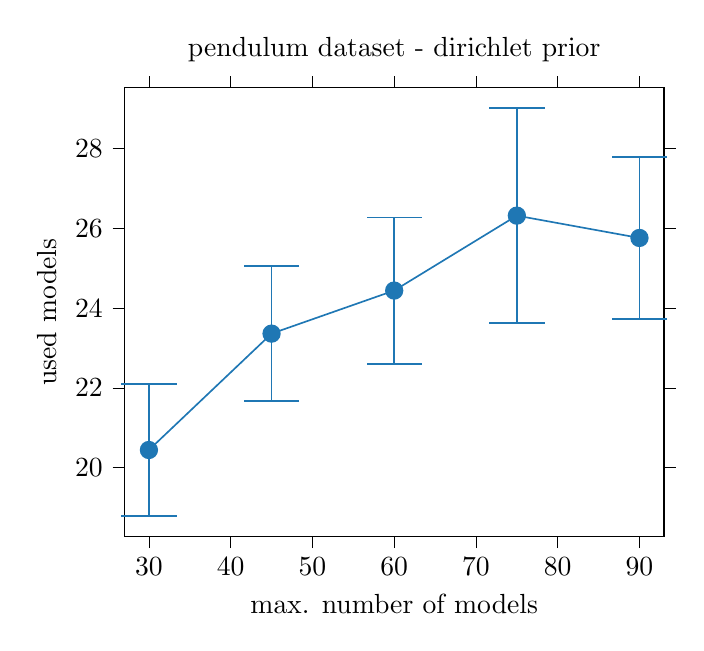
\begin{tikzpicture}

\definecolor{color0}{rgb}{0.12156862745098,0.466666666666667,0.705882352941177}

\begin{axis}[
tick align=outside,
tick pos=both,
title={pendulum dataset - dirichlet prior },
x grid style={white!69.01960784313725!black},
xlabel={max. number of models},
xmin=27, xmax=93,
xtick style={color=black},
y grid style={white!69.01960784313725!black},
ylabel={used models},
ymin=18.2775598690699, ymax=29.5252520541633,
ytick style={color=black}
]
\path [draw=color0, semithick]
(axis cs:30,18.788818604756)
--(axis cs:30,22.091181395244);

\path [draw=color0, semithick]
(axis cs:45,21.6657745132362)
--(axis cs:45,25.0542254867638);

\path [draw=color0, semithick]
(axis cs:60,22.6052248094112)
--(axis cs:60,26.2747751905888);

\path [draw=color0, semithick]
(axis cs:75,23.6260066815228)
--(axis cs:75,29.0139933184772);

\path [draw=color0, semithick]
(axis cs:90,23.7345617758125)
--(axis cs:90,27.7854382241875);

\addplot [semithick, color0, mark=-, mark size=10, mark options={solid}, only marks]
table {%
30 18.788818604756
45 21.6657745132362
60 22.6052248094112
75 23.6260066815228
90 23.7345617758125
};
\addplot [semithick, color0, mark=-, mark size=10, mark options={solid}, only marks]
table {%
30 22.091181395244
45 25.0542254867638
60 26.2747751905888
75 29.0139933184772
90 27.7854382241875
};
\addplot [semithick, color0, mark=*, mark size=3, mark options={solid}]
table {%
30 20.44
45 23.36
60 24.44
75 26.32
90 25.76
};
\end{axis}

\end{tikzpicture}
